\section{Extensions and Robustness}

\subsection{Comparative Statics and Robustness Analysis}

To explore the model's predictions and verify its robustness, we conduct a numerical analysis of how the optimal bias $b^*$ responds to changes in key parameters. The results, summarized in Figure \ref{fig:robustness}, confirm our main theoretical propositions and yield additional, empirically testable insights.

\begin{figure}[H]
    \centering
    % The path is relative from the 'sections' folder up to the project root, then down to 'figures'
    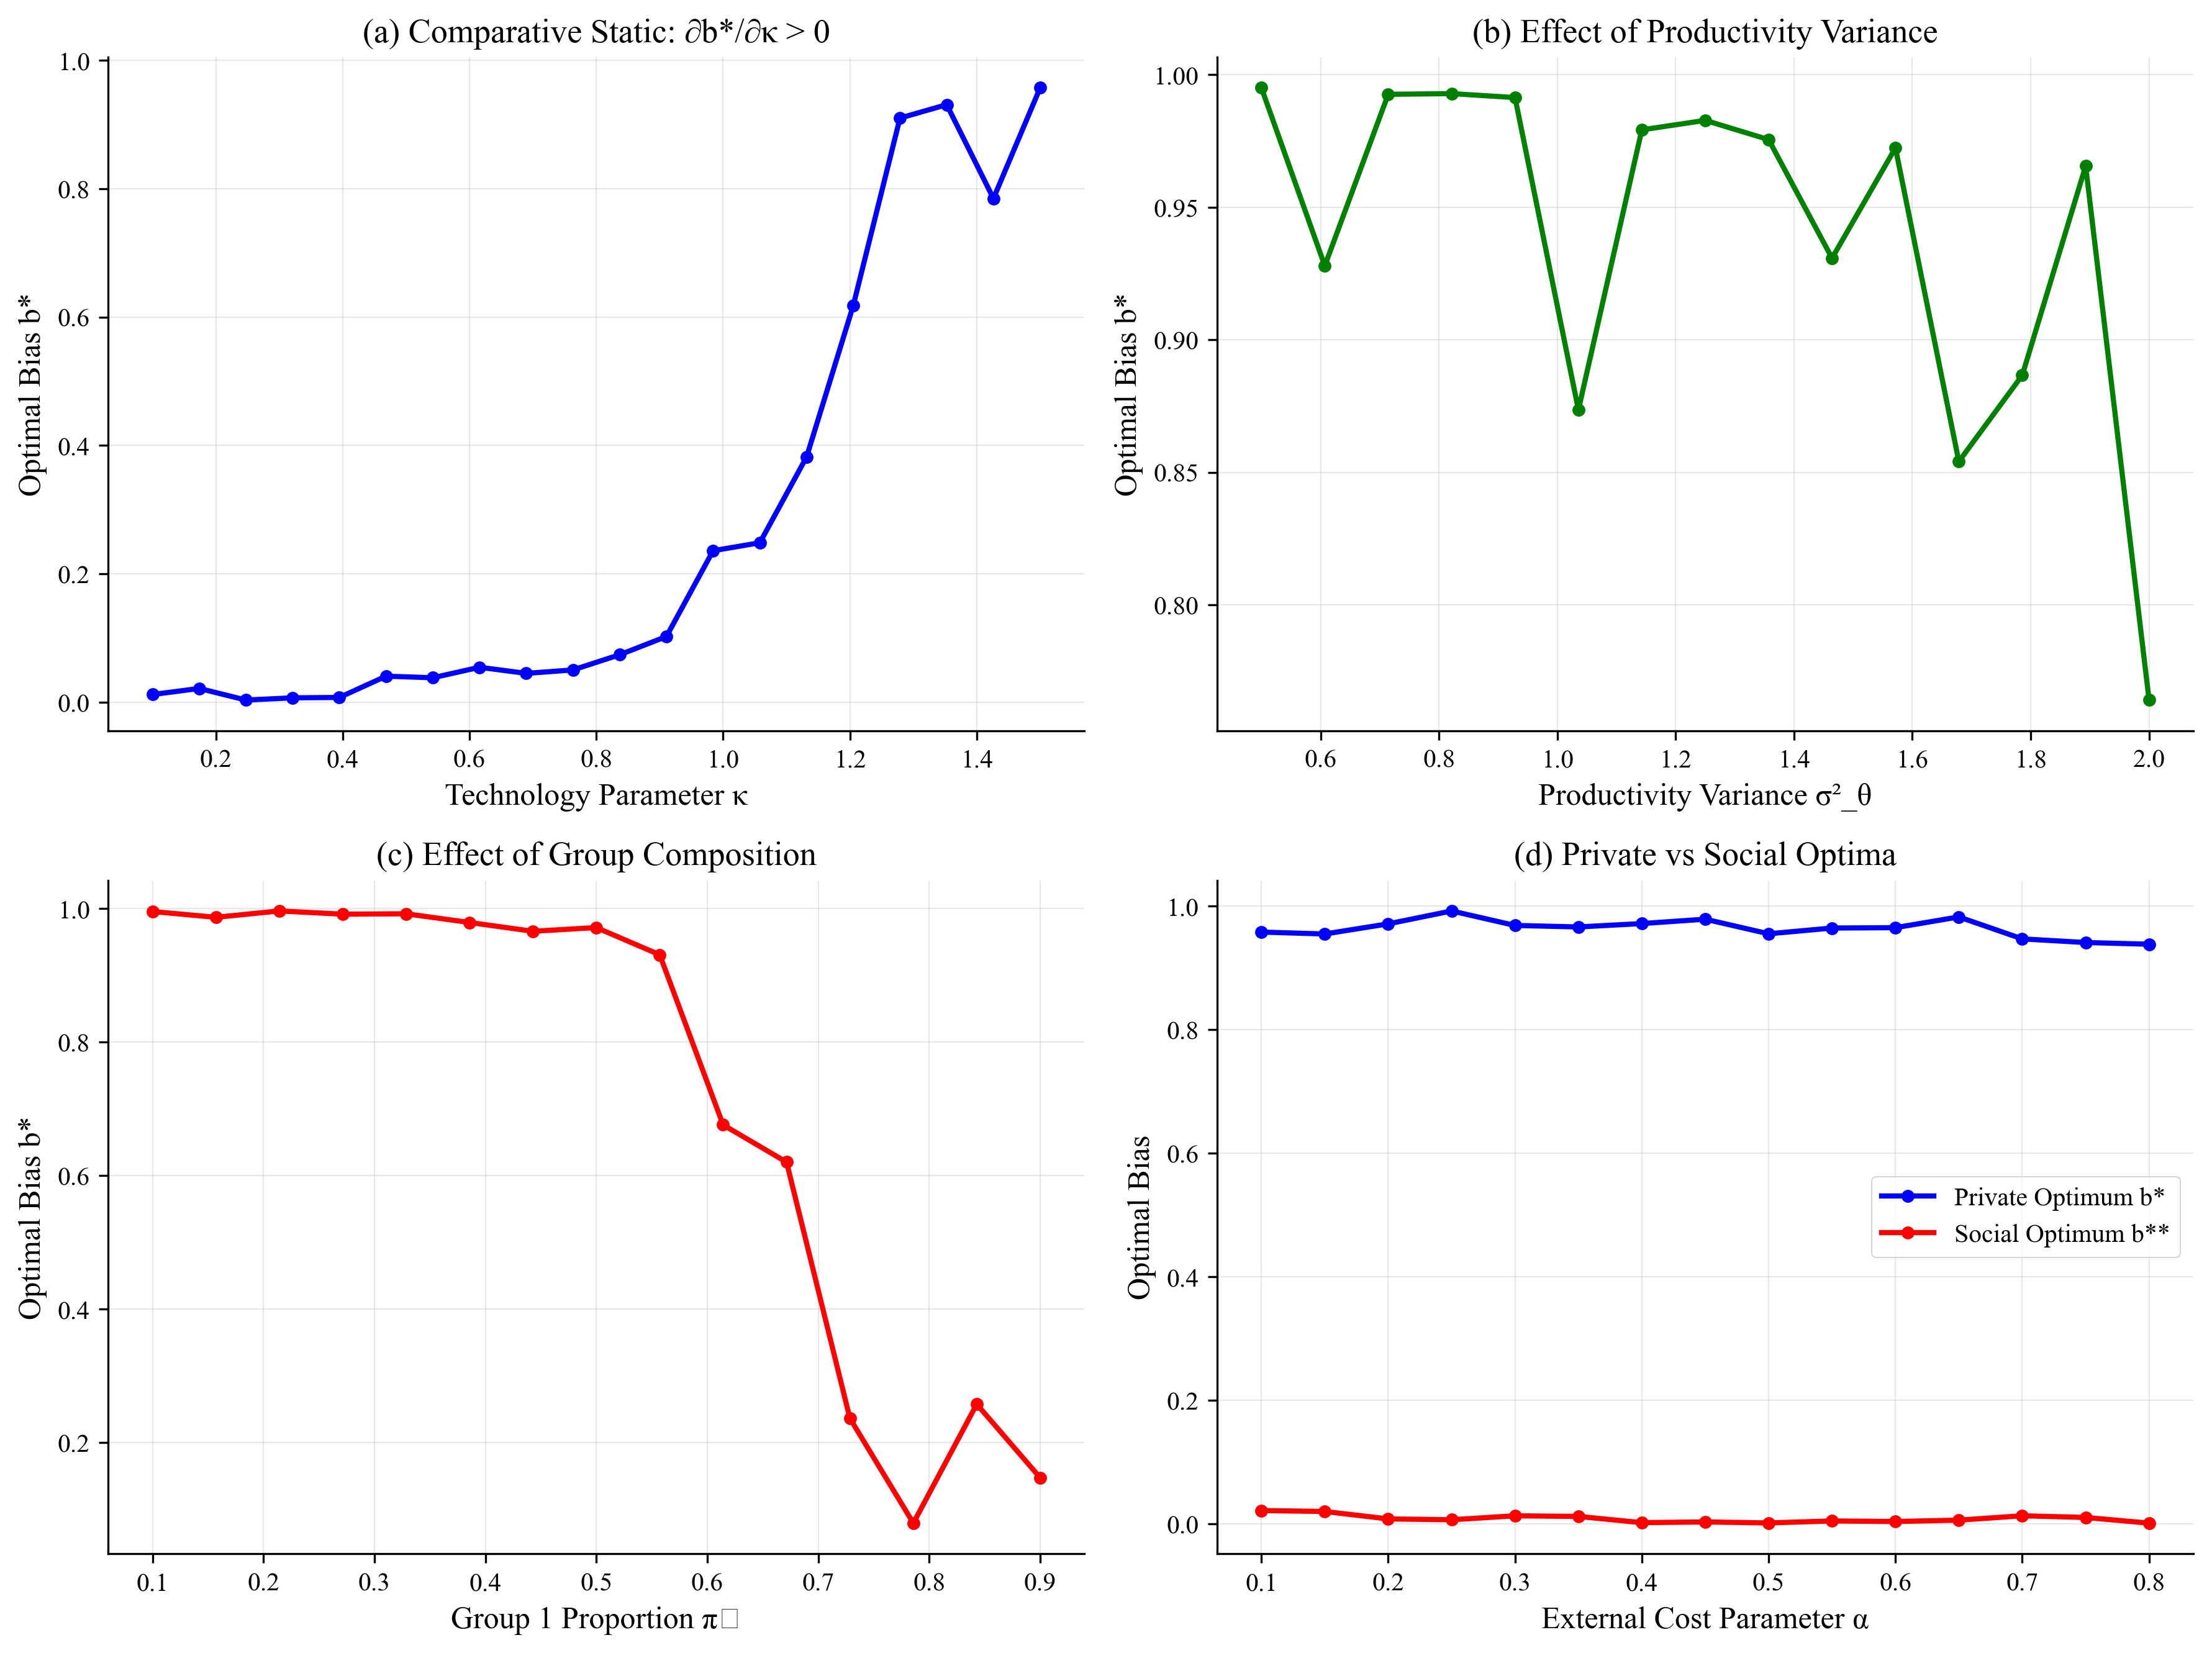
\includegraphics[width=\textwidth]{../figures/figure_robustness.png}
    \caption[Robustness and Comparative Statics]{\textbf{Robustness and Comparative Statics.} 
    Panel (a) numerically confirms Proposition \ref{prop:comparative_static}: optimal bias $b^*$ is increasing in the severity of the trade-off, $\kappa$.
    Panel (b) shows that $b^*$ is largely insensitive to changes in underlying productivity variance $\sigma^2_\theta$.
    Panel (c) reveals that the firm chooses less bias as the disadvantaged group's population share, $\pi_1$, increases.
    Panel (d) illustrates the persistent gap between the private optimum $b^*$ and the social optimum $b^{**}$ across varying levels of external costs.}
    \label{fig:robustness}
\end{figure}

\paragraph{Severity of the Trade-off ($\kappa$).} Panel (a) provides a direct numerical confirmation of Proposition \ref{prop:comparative_static}. As the technology coupling parameter $\kappa$ increases, the marginal gain in signal precision from accepting bias becomes larger, inducing the profit-maximizing firm to choose a higher level of $b^*$.

\paragraph{Productivity Variance ($\sigma^2_\theta$).} Panel (b) explores the effect of underlying talent heterogeneity. The model predicts that optimal bias is relatively insensitive to the variance of true productivity. When $\sigma^2_\theta$ is already high, the signal-to-noise ratio is inherently low, and the marginal benefit of reducing measurement error via bias is diminished.

\paragraph{Group Composition ($\pi_1$).} Panel (c) offers a novel prediction about group composition. When the disadvantaged group is a small minority (low $\pi_1$), the firm is willing to tolerate a high level of bias, as the cost of signal distortion affects only a small fraction of applicants. However, as the disadvantaged group becomes a larger share of the population, the aggregate cost of this distortion becomes substantial, and the firm rationally chooses to decrease its bias.

\paragraph{External Costs ($\alpha$).} Finally, Panel (d) reinforces the core policy dilemma. The firm's private choice, $b^*$, is invariant to the external social cost of bias, $\alpha$, because the firm does not internalize this cost. This leads to a large and persistent divergence from the socially optimal level of bias, $b^{**}$, highlighting the market failure that necessitates policy intervention.

\subsection{Alternative Structures}
Our model's tractability relies on the additive bias structure. However, the core insight about informational motives for bias is robust to alternative specifications.

\paragraph{Multiplicative Bias.} A model with $s = \theta(1+bg) + \varepsilon$ yields qualitatively similar results. The Informativeness Principle still applies, but the quantitative effects and optimal threshold calculations become more difficult.

\paragraph{Feature Selection Bias.} If bias arises from including a feature that is predictive but also correlated with group status, the firm faces a trade-off between the information gained from the feature and the bias it induces. This creates an isomorphic problem structure.

\subsection{Market Dynamics}
Our static, single-firm model provides a foundation for understanding more involved market interactions.

\paragraph{Oligopoly Competition.} In an N-firm model of simultaneous bias choice, equilibrium outcomes depend on the nature of competition. If firms compete for the same pool of applicants, competition could create a ``race to the bottom" on fairness as firms seek any possible predictive edge. Conversely, if fairness can be used as a competitive advantage to attract talent, firms might differentiate their bias levels.

\paragraph{Candidate Responses.} Candidates are not passive. If a firm's bias $b^*$ becomes known, it can trigger strategic responses such as application decisions or attempts to ``game" the algorithm. These long-run effects could discipline the firm's initial choice of bias.